\section{Results}
\label{sec:results}

\subsection{Baselines and linear regression}

Table~\ref{tab:linear} gives the reference points. Predicting the mean gives an RMSE of 62.4
points, the standard deviation of the target. Knowing only the administrative network already
reduces it to 39.7 points ($R^2 = 0.59$). The linear regression with all the attributes
(variant~A) reaches 34.3 points ($R^2 = 0.70$), so the structural attributes add 5.4 points over
the network alone. Relative to state schools, and conditional on the other attributes, the linear
model adds 84.2 points to private schools, 60.4 to federal schools, and 21.8 to municipal schools.

\begin{table}[htbp]
  \centering
  \caption{Baselines and linear regression variants: mean $\pm$ standard deviation over the five
    folds of the first grouped partition.}
  \label{tab:linear}
  \resizebox{\textwidth}{!}{\begin{tabular}{llll}
\toprule
Model & RMSE & MAE & $R^2$ \\
\midrule
Baseline: mean & 62.41 $\pm$ 1.63 & 50.25 $\pm$ 1.36 & -0.00 $\pm$ 0.00 \\
Baseline: network & 39.73 $\pm$ 1.04 & 30.73 $\pm$ 0.88 & 0.59 $\pm$ 0.00 \\
Linear A (with network) & 34.32 $\pm$ 0.93 & 26.15 $\pm$ 0.54 & 0.70 $\pm$ 0.01 \\
Linear B (without network) & 37.40 $\pm$ 0.81 & 28.30 $\pm$ 0.55 & 0.64 $\pm$ 0.01 \\
Linear C (without network and school meals) & 43.97 $\pm$ 1.34 & 33.63 $\pm$ 0.93 & 0.50 $\pm$ 0.01 \\
\bottomrule
\end{tabular}
}
\end{table}

\subsection{Spot-checking}

Table~\ref{tab:spot} and Figure~\ref{fig:spot} summarize the spot-checking over the 15 grouped
partitions. All the algorithms improve on the mean baseline. The SVR (30.77), the random forest
(30.99), and gradient boosting (31.65) lead, followed by $k$-NN (33.91) and linear regression
(34.24); the unpruned decision tree overfits and is the worst model (43.51). The standard
deviations across partitions, about one point, are small compared with the differences between
the groups of algorithms. The Friedman test rejects the hypothesis that all the algorithms are
equivalent ($\chi^2_F = 73.10$, $p = 2.3 \times 10^{-14}$). The average ranks are 1.07 (SVR),
1.93 (random forest), 3.00 (gradient boosting), 4.20 ($k$-NN), 4.80 (linear), and 6.00 (tree),
and the Nemenyi critical difference is 1.95 (Figure~\ref{fig:cd}). The SVR and the random forest are therefore better
than $k$-NN, linear regression, and the tree, and gradient boosting is better than the tree; the
three leaders cannot be separated from one another.

Since the three leaders are statistically tied, and default hyperparameters can hide an algorithm
that would improve more with tuning, we took all three to the tuning stage instead of only the
top-ranked one. We also tuned the decision
tree, whose poor result was clearly caused by the lack of pruning rather than by the algorithm
itself. The training times per fold (6.5~s for the SVR, 2.2~s for gradient boosting, and 1.1~s for
the random forest, on a 12-core machine) made the nested search feasible for the four algorithms.

\begin{table}[htbp]
  \centering
  \caption{Spot-checking with default hyperparameters: mean $\pm$ standard deviation over the
    $3 \times 5$ grouped partitions, and mean training time per fold.}
  \label{tab:spot}
  \begin{tabular}{llllr}
\toprule
Model & RMSE & MAE & $R^2$ & Train time (s) \\
\midrule
SVR & 30.77 $\pm$ 0.90 & 23.43 $\pm$ 0.62 & 0.76 $\pm$ 0.01 & 6.49 \\
Random Forest & 30.99 $\pm$ 0.90 & 23.63 $\pm$ 0.68 & 0.75 $\pm$ 0.01 & 1.05 \\
Gradient Boosting & 31.65 $\pm$ 0.95 & 24.19 $\pm$ 0.70 & 0.74 $\pm$ 0.01 & 2.20 \\
kNN & 33.91 $\pm$ 1.08 & 25.82 $\pm$ 0.78 & 0.70 $\pm$ 0.01 & 0.03 \\
Linear & 34.24 $\pm$ 1.15 & 26.10 $\pm$ 0.82 & 0.70 $\pm$ 0.01 & 0.04 \\
Decision Tree & 43.51 $\pm$ 1.04 & 33.38 $\pm$ 0.67 & 0.51 $\pm$ 0.02 & 0.18 \\
Baseline: mean & 62.35 $\pm$ 1.85 & 50.20 $\pm$ 1.45 & -0.01 $\pm$ 0.01 & 0.03 \\
\bottomrule
\end{tabular}

\end{table}

\begin{figure}[htbp]
  \centering
  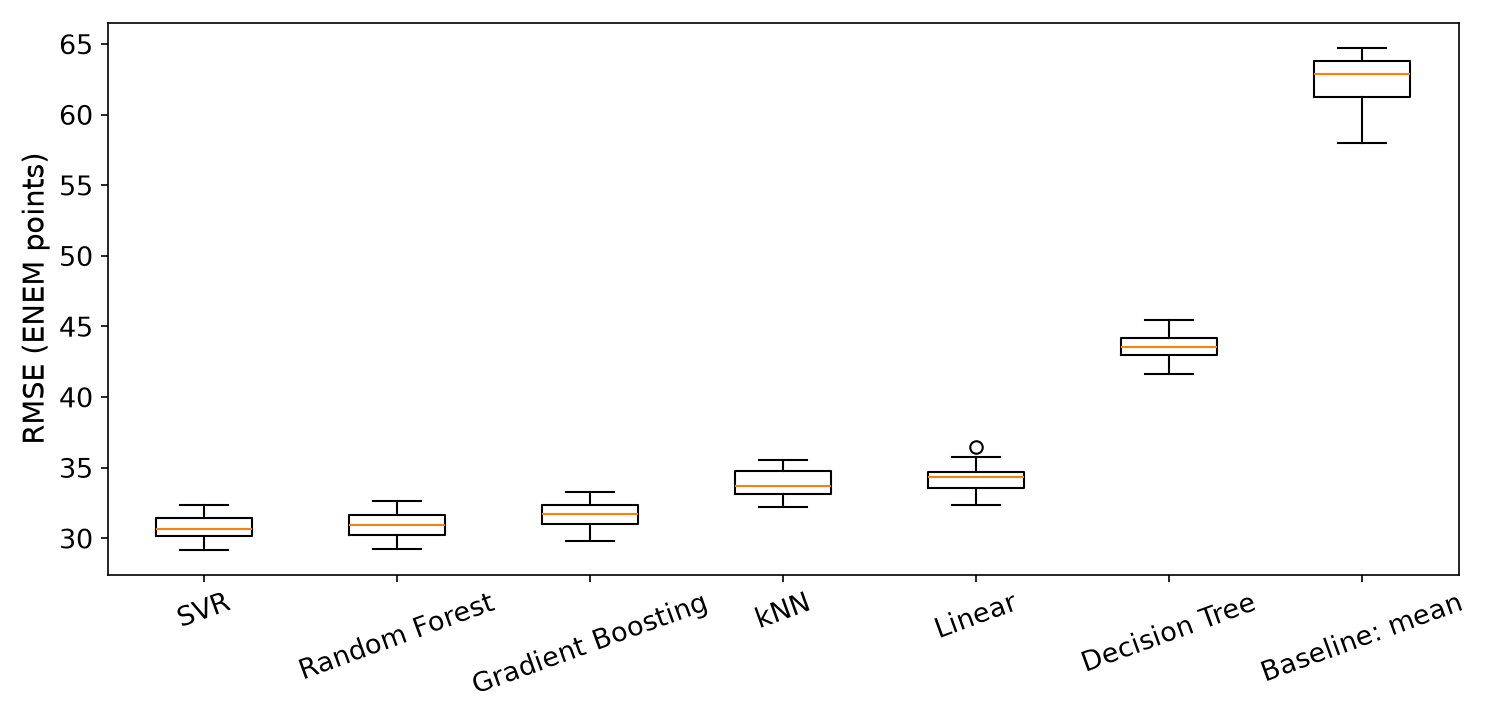
\includegraphics[width=0.9\textwidth]{spot_checking_rmse.png}
  \caption{RMSE of each algorithm over the 15 grouped partitions of the spot-checking.}
  \label{fig:spot}
\end{figure}

\begin{figure}[htbp]
  \centering
  \resizebox{\linewidth}{!}{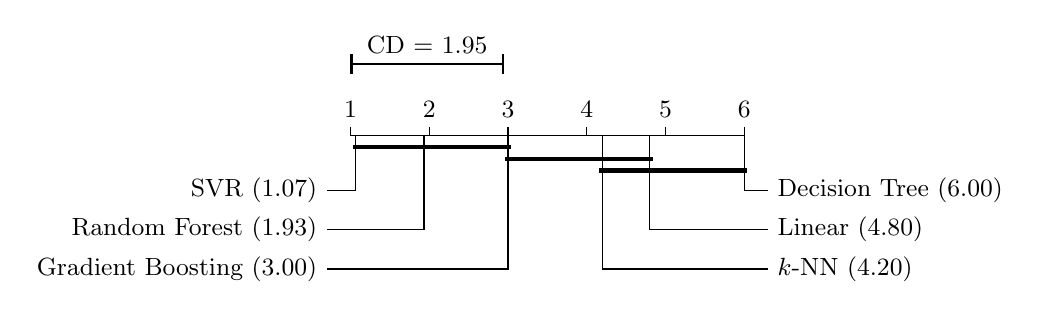
\begin{tikzpicture}[x=1cm,y=1cm,font=\small]
\draw (0,0) -- (5.0,0);
\draw (0.0,0) -- (0.0,0.1) node[above]{1};
\draw (1.0,0) -- (1.0,0.1) node[above]{2};
\draw (2.0,0) -- (2.0,0.1) node[above]{3};
\draw (3.0,0) -- (3.0,0.1) node[above]{4};
\draw (4.0,0) -- (4.0,0.1) node[above]{5};
\draw (5.0,0) -- (5.0,0.1) node[above]{6};
\draw[|-|,thick] (0,0.9) -- (1.947,0.9) node[midway,above]{CD = 1.95};
\draw (0.067,0) -- (0.067,-0.70) -- (-0.3,-0.70) node[left]{SVR (1.07)};
\draw (0.933,0) -- (0.933,-1.20) -- (-0.3,-1.20) node[left]{Random Forest (1.93)};
\draw (2.0,0) -- (2.0,-1.70) -- (-0.3,-1.70) node[left]{Gradient Boosting (3.00)};
\draw (3.2,0) -- (3.2,-1.70) -- (5.3,-1.70) node[right]{$k$-NN (4.20)};
\draw (3.8,0) -- (3.8,-1.20) -- (5.3,-1.20) node[right]{Linear (4.80)};
\draw (5.0,0) -- (5.0,-0.70) -- (5.3,-0.70) node[right]{Decision Tree (6.00)};
\draw[line width=1.6pt] (0.03,-0.15) -- (2.04,-0.15);
\draw[line width=1.6pt] (1.96,-0.30) -- (3.84,-0.30);
\draw[line width=1.6pt] (3.16,-0.45) -- (5.04,-0.45);
\end{tikzpicture}
}
  \caption{Critical-difference diagram of the spot-checking (average ranks over 15 partitions,
    lower is better). Algorithms joined by a bar are not significantly different (Nemenyi,
    $\alpha = 0.05$).}
  \label{fig:cd}
\end{figure}

\subsection{Tuned models}

Table~\ref{tab:tuned} compares the default and tuned versions on the same outer partitions. The
tuning fixes the overfitting of the decision tree, whose RMSE drops by 10.2 points, to 33.31, with
\texttt{max\_depth}$=10$ in all 15 searches. The SVR and the random forest barely change (less than
0.1 point), indicating that their defaults were already close to the best of the grid. Gradient
boosting gains 1.0 point and becomes the best model, with RMSE 30.63 ($R^2 = 0.757$).

\begin{table}[htbp]
  \centering
  \caption{Default vs.\ tuned hyperparameters (nested cross-validation): mean over the
    $3 \times 5$ outer grouped partitions. ``Gain'' is the reduction in RMSE points.}
  \label{tab:tuned}
  \resizebox{\textwidth}{!}{\begin{tabular}{lrrrrrr}
\toprule
Model & RMSE default & RMSE tuned & Std (tuned) & $R^2$ default & $R^2$ tuned & Gain (RMSE) \\
\midrule
Gradient Boosting & 31.654 & 30.634 & 0.898 & 0.741 & 0.757 & 1.020 \\
SVR & 30.770 & 30.676 & 0.892 & 0.755 & 0.756 & 0.094 \\
Random Forest & 30.989 & 30.905 & 0.893 & 0.751 & 0.753 & 0.084 \\
Decision Tree & 43.514 & 33.313 & 0.884 & 0.510 & 0.713 & 10.201 \\
\bottomrule
\end{tabular}
}
\end{table}

The selected hyperparameters were stable: gradient boosting chose \texttt{learning\_rate}$=0.05$
and \texttt{max\_depth}$=5$, and the SVR chose $C=1$ and $\varepsilon=0.3$, in all 15 outer folds;
the random forest chose \texttt{max\_depth}$=20$ in all 15, with \texttt{min\_samples\_leaf}$=1$ in
12. Some of these choices lie on the border of the grid (the smallest learning rate and largest
depth for gradient boosting, the smallest $C$ and largest $\varepsilon$ for the SVR), so a wider
grid could improve them further.

The Friedman test again rejects the null hypothesis ($\chi^2_F = 37.64$, $p = 3.4 \times
10^{-8}$). The average ranks are 1.40 (gradient boosting), 1.73 (SVR), 2.87 (random forest), and
4.00 (tree), with a critical difference of 1.21: gradient boosting and the SVR are better than the
tree, and gradient boosting is better than the random forest, but gradient boosting and the SVR
cannot be separated. In absolute terms, the three best models are within 0.3 RMSE points of each
other, a difference that is small on the ENEM scale. We selected gradient boosting for the
interpretation because it has the lowest error and the best average rank, and because tree
ensembles admit exact and fast SHAP values, which the SVR does not. The whole nested
cross-validation took about 17 minutes.